\documentclass{ximera}

\title{Implicit Differentiation Activity}
\author{MATH 425: Calculus I}

\begin{document}
\begin{abstract}
    Working with the peers in your group, solve the following problems. Make sure to show and justify all your work. Make sure everyone in the group understands the solution and participates. Be prepared to report your answers to the whole class. 
\end{abstract}
\maketitle


\begin{exercise}
    Consider the curve on the graph and the equation of the curve: 
    $$x=y^5-5y^3+4y.$$
    With your group, explain how you would answer the following questions, using both the graph of the curve and the symbolic equation.
    \begin{image}
    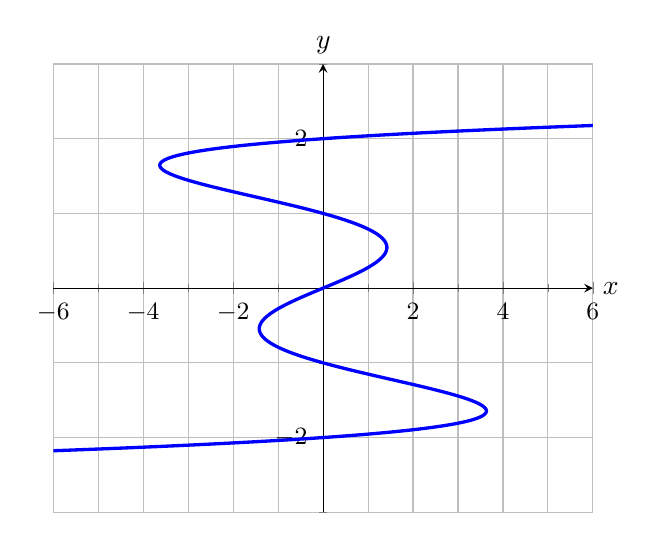
\begin{tikzpicture}
  \begin{axis}[
    axis lines=middle,
    xlabel={$x$},
    ylabel={$y$},
    xmin=-6, xmax=6,
    ymin=-3, ymax=3,
    grid=both,
    minor tick num=1,
    enlargelimits=false,
    ticklabel style={font=\small},
    every axis x label/.style={at={(current axis.right of origin)}, anchor=west},
    every axis y label/.style={at={(current axis.above origin)}, anchor=south},
  ]

    \addplot[
      domain=-2.5:2.5,
      samples=500,
      very thick,
      blue
    ] ({x^5 - 5*x^3 + 4*x}, {x});

  \end{axis}
\end{tikzpicture}
    \end{image}
  \begin{enumerate}
    \item Is it possible to express $y$ as an explicit function of $x$?  
    \begin{enumerate}
        \item Explain your response using the graph.
        \item Explain using the symbolic equation for the curve $x=y^5-5y^3+4y$.
    \end{enumerate}
    \item Use implicit differentiation to find a formula for $\frac{dy}{dx}$.  
    \item Explain the meaning of $\frac{dy}{dx}$.  What does it represent?
    \item Sam noticed that his expression for $\frac{dy}{dx}$ does not contain $x$.  Sam thinks this means that the rate of change is constant for all points on the $x$-axis.  Is Sam correct in his thinking or not? Explain.
    \item Find the equation of the line tangent to the graph of $x=y^5-5y^3+4y$ at the point $(0,1)$.  Add a sketch of the tangent line to the graph.
    \item Are there other points on the graph where the tangent line is the same as you found in (e)?  Respond using the graph, then verify algebraically.
    \item Determine all points at which the graph of $x=y^5-5y^3+4y$ has a vertical tangent line.  How many such points are there?  Explain your reasoning, and locate the points on the graph.
  \end{enumerate}
\end{exercise}

Problem adapted from Boelkins, Austin \& Schlicker, (2018) \textit{Active Calculus 2.1}.

\begin{exercise}
  Consider the expression $x^2+xy+y^2=3$. 
    \begin{center}
      \desmos{yey6o1coa2}{800}{600}
    \end{center}
    \begin{enumerate}
      \item Use implicit differentiation to find $y'$ (also known as $\frac{dy}{dx}$).  
      \item Find the tangent line to $x^2+xy+y^2=3$ at the point $(-1,-1)$.  Sketch the tangent line on the graph (in Desmos) and check your equation is consistent with what you expect.  
      \item Find any points where the tangent line to the curve is horizontal using the graph.  Sub these points into the derivative to confirm the result.
    \end{enumerate}
\end{exercise}

%\begin{exercise}
%    Consider the equation whose graph is given below: 
%    $$y(y^2-1)(y-2)=x(x-1)(x-2)$$
%   \[ \graph{y(y^2-1)(y-2)=x(x-1)(x-2)}   \]
% Need a workaround for PDF version
%   \begin{enumerate}
%     \item Examine the graph of the curve and determine at how many points the tangent to the curve is horizontal.  Add the sketch of the horizontal tangent lines to the graph. 
%     \item Through implicit differentiation, it can be shown that 
%       $$\frac{dy}{dx}=\frac{(x-1)(x-2)+x(x-2)+x(x-1)}{(y^2-1)(y-2)+2y^2(y-2)+y(y^2-1)}$$
%       Determine all $x$-values at which the tangent line to the curve is horizontal.  Compare the result of your calculation to the answer you got in question (a).
%     \item Determine all the points $(x,y)$ at which the tangent line to the curve is vertical.  You may use a graphing calculator or Desmos for this. 
%     \item Find the equation of the tangent line to the curve at one of the points where $x=1$.
%   \end{enumerate}
% \end{exercise}

% Problems adapted from Boelkins, Austin \& Schlicker, (2018) \textit{Active Calculus 2.1}.





\end{document}
